\documentclass{article}
\usepackage{graphicx}

\graphicspath{{./img/}}
\title{2411 HW 4}
\author{Duncan Wilkie}
\date{1 October 2021}

\begin{document}

\maketitle

\section{}
The program appears in the Script Files section. The resulting plot of its output is immediately below.
\[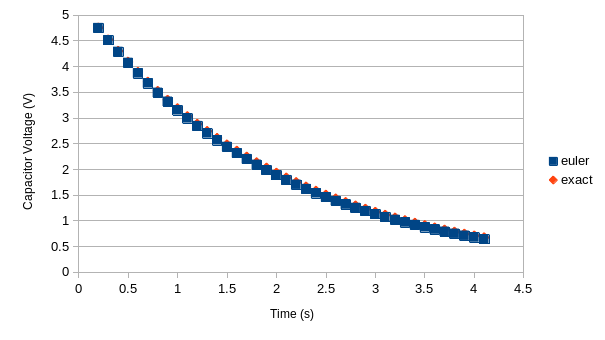
\includegraphics[scale=0.5]{plot1.png}\]
This shows quite good agreement between the exact result and Euler's algorithm, with a small accumulating undershoot in the computed values.

\section{}
\[\frac{dy}{dx}\bigg|_{x_0} = \frac{y(t_{n+1})-y(t_n)}{h}-O\left(\frac{h}{2}\frac{d^2y}{dx^2}\bigg|_{x_0}\right)=f(t,y)\]
\[\Rightarrow y_{n+1}=y+hf(t,y) + hO\left(\frac{h}{2}\frac{d^2y}{dx^2}\bigg|_{x_0}\right)\]
\[= y+hf(t,y) + O\left(\frac{h^2}{2}\frac{d^2y}{dx^2}\bigg|_{x_0}\right)\]
The absolute approximation error is this rightmost summand.

\section{}
We perform one Euler step to find $\frac{dx}{dt}$ at $t=0.2$:
\[\frac{dx}{dt}\bigg|_{0.2}=\frac{dx}{dt}\bigg|_{0}+(0.2)h=50.04\]
This enables us to perform the Euler step to find $x$:
\[x(0.2)=x(0)+(0.2)(50.04)=20.008\]
\section{}
The program appears in the Script Files section. The resulting plot appears below.
\[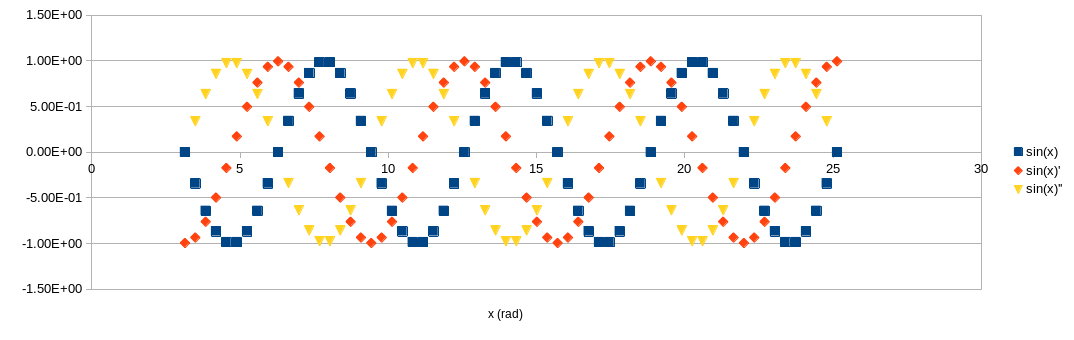
\includegraphics[scale=0.4]{plot2.png}\]
This is consistent with the analytical solutions, since the amplitudes are identical and the phases are a quarter wavelength for each differentiation.
The output for a few selected points appears below.
\begin{center}
  \begin{tabular}{ |c|c|c|c|c| }
    \hline
    $x$ (deg) & $x$ (rad) & $\sin(x)$ & $\sin(x)'$ & $\sin(x)''$ \\
    \hline \hline
    3.14159 & 180 & 1.22465e-16 & -0.994931 & 6.36111e-16 \\
    \hline
    4.71239&	270&	-1&	-2.54E-15&	0.997464\\
    \hline
    6.28319 & 360 & -2.90946e-15 & 0.994931 & 2.54444e-15 \\
    \hline
    7.85398&	450&	1&	5.09E-15&	-0.997464\\
    \hline

    
  \end{tabular}
\end{center}
These values appear to be correct to the second place in general, with much better agreement in specific cases. 
The disagreement in the peak points when compared to the precision of the points corresponding to the zeroes is due to the dependence of the approximation error on the value of $f^3$ at the point in question---the approximation error is zero when $f^3$ is zero, and is highest whenever $f^3$ is highest, under the assumption of fixed $h$. 
\section{}
The program appears in the Script Files section. The resulting plot appears below.
\[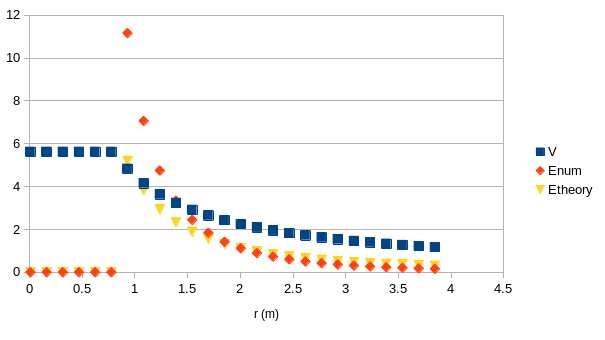
\includegraphics[scale=0.5]{plot3.png}\]
It appears that the discontinuity affects the accuracy of the extrapolated difference method, with high computational errors observed to the point that the computed solution appears to be in downright disagreement with the theoretical value.
\section*{Script Files}
\subsection*{Program 1}
\begin{verbatim}
Script started, file is dwilk14_hw4p1.txt
[dwilk14@tigers ~/HW4]$ cat dwilk14_hw4p1.cpp
#include <cmath>
#include <iostream>
#include <fstream>
#include <cstdlib>

using namespace std;

struct array {double *vals; int size;};

array euler(double (*f)(double), double a, double b, double y_0, double h) { // implementation for dy/dt = f(y)
  double y = y_0;
  int n = (b - a) / h;
  double *result = (double*)malloc(n * sizeof(double));

  for (int i = 0; i < n; i++) {
    y += h * f(y);
    result[i] = y;
  }

  array r = {result, n};
  return r;

}

double f(double V) {
  return -V / 2;
}

double exact(double t) {
  return 5 * exp(-t / 2);
}
int main() {
  ofstream outfile;
  outfile.open("output.txt");
  array result = euler(f, 0, 4, 5, 0.1);
  double t = 0.1;
  for (int i = 0; i < result.size; i++) {
    t += 0.1;
    outfile << t << " " << result.vals[i] << " " << exact(0.1 + i * 0.1)<< endl;
  }

  return 0;

}
[dwilk14@tigers ~/HW4]$ g++ dwilk14_hw4p1.cpp -o dwilk14_hw4p1
[dwilk14@tigers ~/HW4]$ ./dwilk14_hw4p1
[dwilk14@tigers ~/HW4]$ cp dwilk14_hw4p1.txt /home3/kristina/phys2411/.
[dwilk14@tigers ~/HW4]$ exit
exit
Script done, file is dwilk14_hw4p1.txt
\end{verbatim}
\subsection*{Program 2}
\begin{verbatim}
Script started, file is dwilk14_hw4p2.txt
[dwilk14@tigers ~/HW4]$ cat dwilk14_hw4p2.cpp
#include <cmath>
#include <fstream>
#include <iostream>

using namespace std;

double cd(double (*f)(double), double x, double h) {
  return (f(x + h / 2) - f(x - h / 2)) / h;
}

double c2d(double (*f)(double), double x, double h) {
  return (cd(f, x + h / 2, h) - cd(f, x - h / 2, h)) / h;
}

int main() {
  ofstream outfile;
  outfile.open("output2");
  double x = M_PI, end = 8 * M_PI, h = M_PI / 18;

  outfile << "x[rad] x[deg] sin(x) sin(x)' sin(x)''" << endl;

  while (x < end) {
    outfile << x << " " << x * 180 / M_PI << " " << sin(x) << " " \
         << cd(sin, x, h) << " " << c2d(sin, x, h) << endl;
    x += h;
  }

  return 0;

}
[dwilk14@tigers ~/HW4]$ g++ dwilk14_hw4p2.cpp -o dwilk14_hw4p2
[dwilk14@tigers ~/HW4]$ ./dwilk14_hw4p2
[dwilk14@tigers ~/HW4]$ cp dwilk14_hw4p2.txt /home3/kristina/phys2411/.
[dwilk14@tigers ~/HW4]$ exit
exit
Script done, file is dwilk14_hw4p2.txt
\end{verbatim}
\subsection*{Program 3}
\begin{verbatim}
Script started, file is dwilk14_hw4p3.txt
[dwilk14@tigers ~/HW4]$ cat dwilk14_hw4p3.cpp
#include <cmath>
#include <fstream>
#include <iostream>

using namespace std;

double ed(double (*f)(double), double x, double h) {
  return 1 / (3 * h) * (8 * (f(x + h/4) - f(x - h/4)) - (f(x + h/2)-f(x - h/2)));
}

double V(double r) {
  return (r > 0.8) ? 4.5 / r : 5.625;
}

double E(double r) {
  return (r > 0.8) ? 4.5 / pow(r, 2) : 0;
}

int main() {
  ofstream outfile;
  outfile.open("output3.txt");
  double h = 0.02, r = 0.01, b = 4, step = (b - r) / 26;

  outfile << "r V Enum Etheory" << endl;
  for (int i = 0; i < 26; i++) {
    outfile << r << " " <<  V(r) << " " <<  -ed(E, r, h) << " " << E(r) << endl;
    r += step;
  }

  return 0;
  
}
[dwilk14@tigers ~/HW4]$ g++ dwilk14_hw4p3.cpp -o dwilk14_hw4p3
[dwilk14@tigers ~/HW4]$ ./dwilk14_hw4p3
[dwilk14@tigers ~/HW4]$ cp dwilk14_hw4p3.txt /home3/kristina/phys2411/.
[dwilk14@tigers ~/HW4]$ exit
exit
Script done, file is dwilk14_hw4p3.txt
\end{verbatim}
\end{document}
%%% Local Variables:
%%% mode: latex
%%% TeX-master: t
%%% End:
